%Part of/Parte di https://github.com/f-dinucci/appuntiMeccanicaFluidi/
%License/Licenza Creative Commons Attribution-ShareAlike 4.0 International (CC BY-SA 4.0) - attribution/attribuzione Francesco Di Nucci
%See also/Vedere anche https://creativecommons.org/licenses/by-sa/4.0/ and/e https://creativecommons.org/licenses/by-sa/4.0/legalcode
%
\section{Flusso irrotazionale}
\subsection{Corrente a potenziale}
Le equazioni di Eulero non sono un problema lineare, ma si può arrivare ad una sola equazione.
%
	\begin{equation*}
		\begin{gathered}
			\div{\uline{v}} = 0\\
			\curl{\uline{v}} = \uline{\omega} = 0
		\end{gathered}
	\end{equation*}
%
Si introduce un potenziale per la velocità, per il rotore nullo di un campo vettoriale il potenziale è uguale al gradiente di uno scalare:
%
	\begin{equation*}
		\uline{v} = \grad{\phi}
	\end{equation*}
%
Si introduce quindi l'equazione di Laplace:
%
	\begin{equation*}
		\div{\grad{\phi}} = \laplacian{\phi} = 0
	\end{equation*}
%
Nel caso bidimensionale si arriva quindi a scrivere:
%
	\begin{equation*}
		\phi_{xx} + \phi_{yy} = 0
	\end{equation*}
%
Questa permette una soluzione a variabili separabili, si ipotizza:
%
	\begin{equation*}
		\phi(x,y) = F(x) G(y)
	\end{equation*}
%
Quindi:
%
	\begin{equation*}
		\begin{gathered}
			F_{xx} G + F G_{yy} = 0\\
			\frac{F_{xx}}{F} = - \frac{G_{yy}}{G} = C\\
			F_{xx} = CF; \quad G_{yy} = - CG
		\end{gathered}
	\end{equation*}
%
Sono equazioni a coefficienti costanti, hanno una soluzione esponenziale:
%
	\begin{equation*}
		\begin{gathered}
			F = e^{ax} \rightarrow a^2 F = C F \rightarrow a^2 = C\\
			G = e^{by} \rightarrow b^2 G = - C G \rightarrow b^2 = -C = -a^2
		\end{gathered}
	\end{equation*}
%
Ne risulta una soluzione a valori complessi, parte reale e immaginaria obbediscono alla stessa legge, è possibile prenderne solamente una parte e comunque sarà una soluzione valida.
Si prende $a$ reale tale che:
%
	\begin{equation*}
		\begin{gathered}
			b = \pm ia\\
			\phi = e^{ax} e^{\pm iay}
		\end{gathered}
	\end{equation*}
%
Dato che $a$ è un parametro libero, è una famiglia di soluzioni.
Noto questo è possibile risolvere una serie di problemi.

%SUBSECTION
\subsection{Lastra verticale} 
Nel caso di una lastra verticale occorre scegliere l'esponenziale con il segno giusto, che deve andare a zero dal lato del moto del fluido.
 %
	\begin{figure}[ht]
		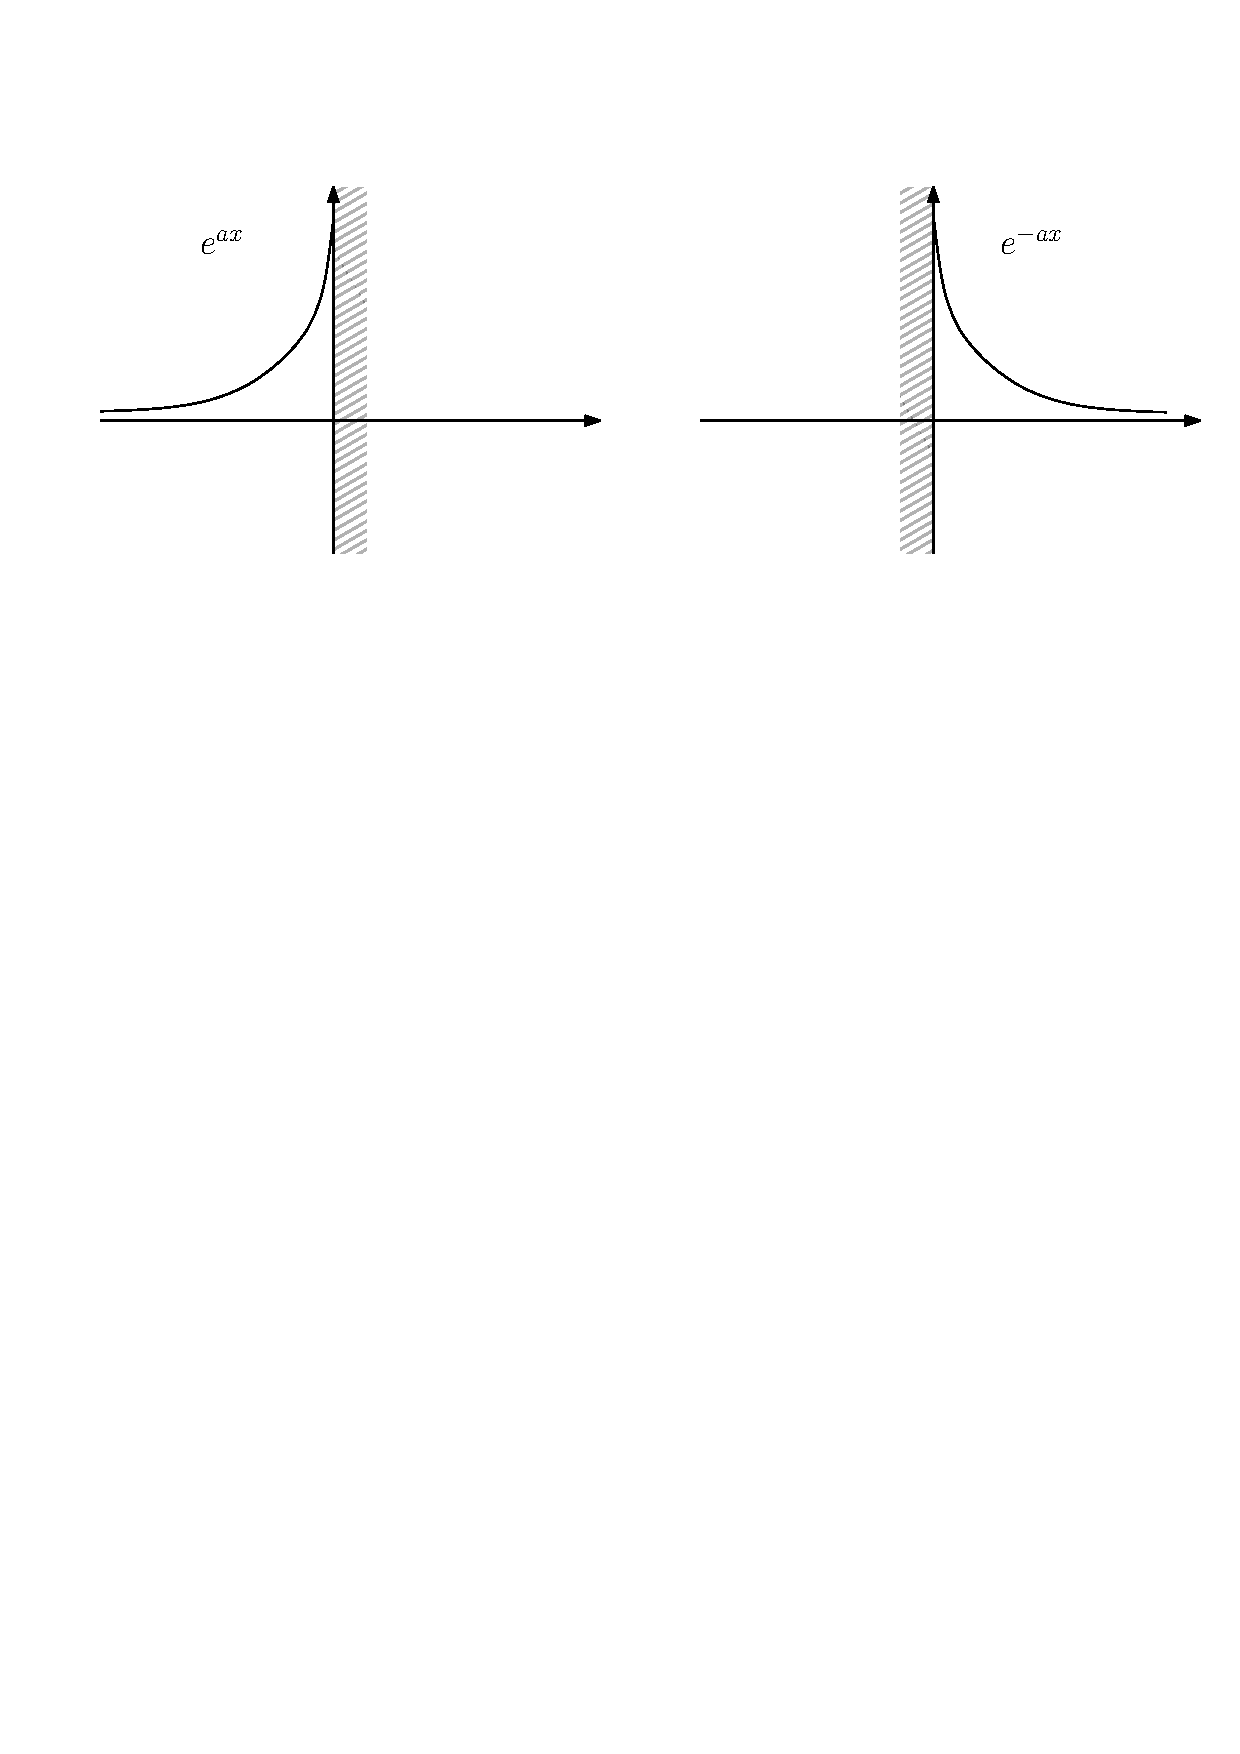
\includegraphics[scale=0.6]{./7.3 Flusso irrotazionale/7.3-1}
		\centering
		\caption{Esponenziale e lastra verticale}
	\end{figure}
%
È interessante portare il problema in coordinate cilindriche:
%
	\begin{equation*}
		\begin{gathered}
			\laplacian{\phi} = 0\\
			\frac{1}{r} \pdv{r} \left( r \pdv{\phi}{r} \right) + \frac{1}{r^2} \pdv[2]{\phi}{\theta} = 0
		\end{gathered}
	\end{equation*}
%
Si ipotizza che la soluzione sia prodotto di due funzioni:
%
	\begin{equation*}
		\begin{gathered}
			\phi = F(r) G(\theta)\\
			\frac{1}{r} \pdv{r} \left( r \pdv{F}{r} \right) G + \frac{F}{r^2} \pdv[2]{G}{\theta} = 0
		\end{gathered}
	\end{equation*}
%
Separando le variabili:
%
	\begin{equation*}
		\begin{gathered}
			\frac{1}{F} r \pdv{r} \left( r \pdv{F}{r} \right) = - \frac{1}{G} \pdv[2]{G}{\theta} = C\\
			r \pdv{r} \left( r \pdv{F}{r}\right) = CF; \quad \pdv[2]{G}{\theta} = - CG
		\end{gathered}
	\end{equation*}
%
La seconda è un'equazione differenziale a coefficienti costanti:
%
	\begin{equation*}
		\begin{gathered}
			G = e^{b \theta}\\
			b^2 = - C
		\end{gathered}
	\end{equation*}
%
La prima invece è omogenea:
%
	\begin{equation*}
		\begin{gathered}
			F = r^{\theta}\\
			r \pdv{r} ( a r^a ) = a^2 r^a \rightarrow a^2 = C = -b^2
		\end{gathered}
	\end{equation*}
%
Per motivi fisici la soluzioni deve essere periodica di $\theta$: in coordinate cilindriche effettuando una rotazione completa si torna al punto di partenza, quindi le funzioni devono essere periodiche, altrimenti nello stesso punto si avrebbero due valori diversi.
%
	\begin{figure}[ht]
		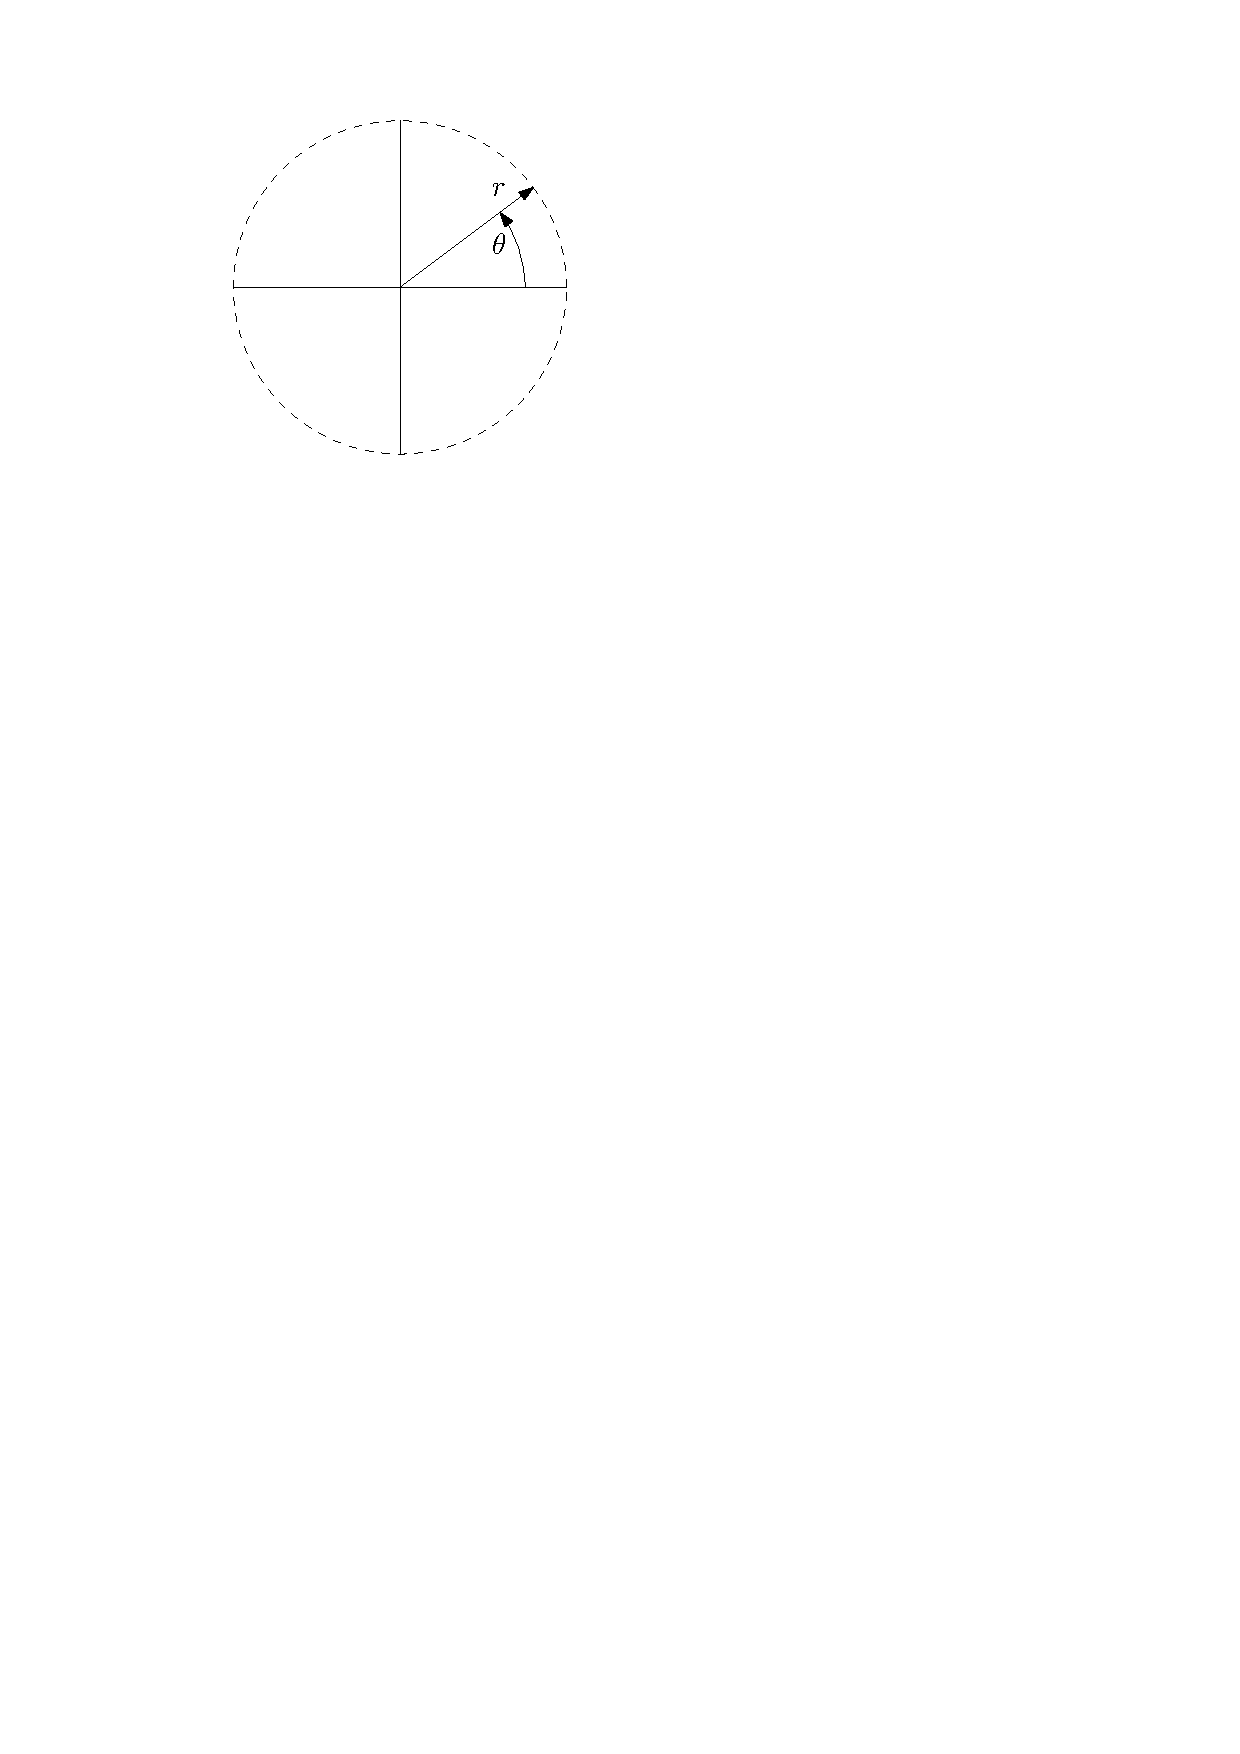
\includegraphics[scale=0.7]{./7.3 Flusso irrotazionale/7.3-2}
		\centering
		\caption{Periodicità in coordinate cilindriche}
	\end{figure}
%
Quindi $G(\theta)$ è periodica di periodo $2 \pi$.
Questo capita se $b$, oltre ad essere un immaginario puro, è un numero intero.
Applicando la formula di Eulero si vede che:
%
	\begin{equation*}
		\begin{gathered}
			e^{i \theta} = \cos{\theta} + i \sin{\theta}\\
			b = in\\
			a = \pm  n			
		\end{gathered}
	\end{equation*}
%
È una sequenza di soluzioni.

Per $n = 0$, si ha che $\phi = A$, ma è strano poiché l'equazione di Laplace è lineare del secondo ordine, deve avere due soluzioni indipendenti con cui costruire le altre.
Si vede però che:
%
	\begin{equation*}
		\begin{gathered}
			A = 0 \rightarrow C = 0\\
			\frac{1}{r} \pdv{r} \left( r \pdv{F}{r} \right) = 0 \rightarrow r \pdv{F}{r} = B = cost.\\
			\pdv{F}{r} = \frac{B}{r} \rightarrow F = B \log{r} + A
		\end{gathered}
	\end{equation*}
%
È una soluzione con due parametri indipendenti, per G si effettua lo stesso ragionamento:
%
	\begin{equation*}
		\begin{gathered}
			\pdv[2]{G}{\theta} = 0 \rightarrow G = A + B \theta
		\end{gathered}
	\end{equation*}
%
Questa non è periodica, ma le sue derivate sì (inclusa la velocità).
Questo è sufficiente, dato che il potenziale $\phi$ è un ente fittizio, il ragionamento fisico si applica alle proprietà che sono sue derivate.

%SUBSECTION
\subsection{Studio della sequenza di soluzioni}
\subsubsection{Fluido fermo}
Come caso particolare risulta il fluido fermo:
%
	\begin{equation*}
		\phi = A \rightarrow \grad{\phi} = 0
	\end{equation*}
%

\subsubsection{Pozzo/sorgente}
%
	\begin{equation*}
		\phi = b \log{r} \rightarrow \grad{\phi} = B \frac{1}{r} \hat{\imath}_r
	\end{equation*}
 %
	\begin{figure}[ht]
		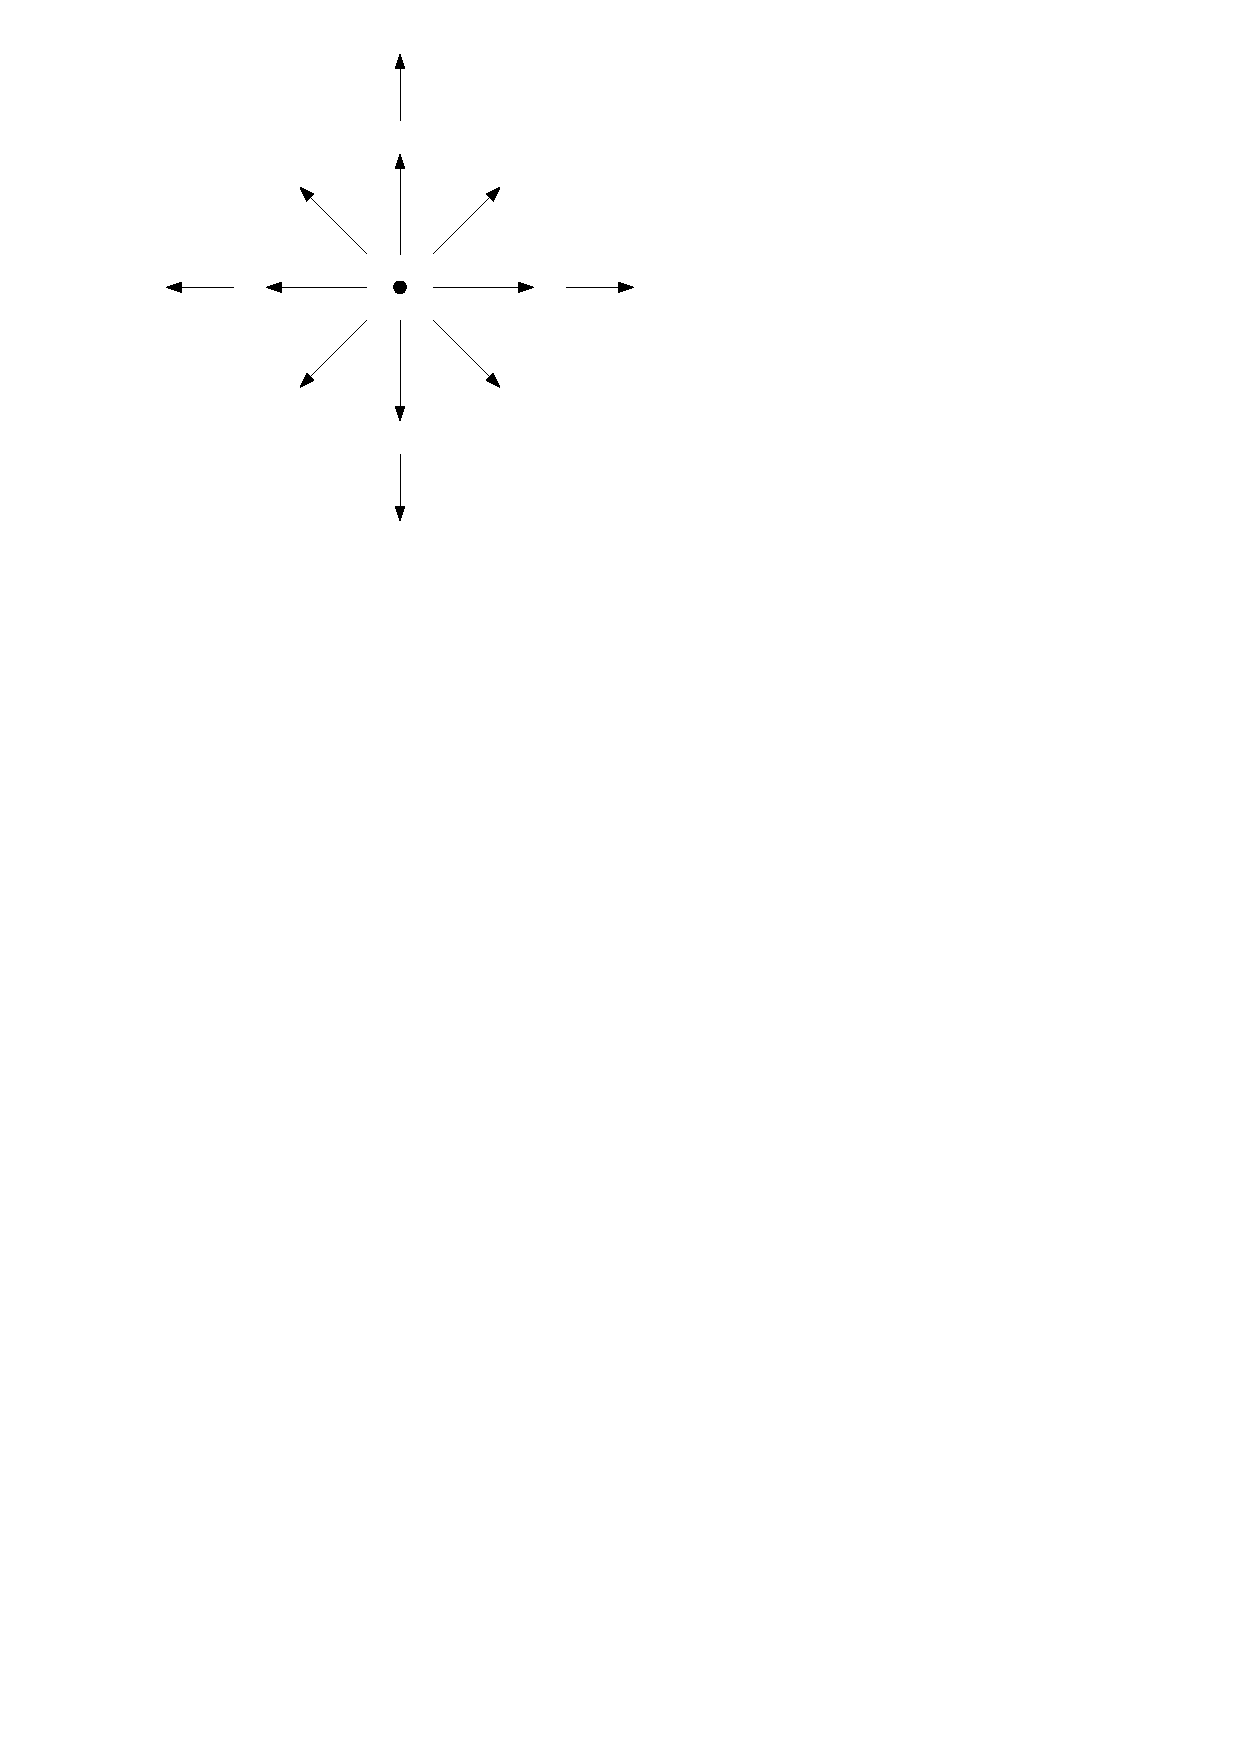
\includegraphics[scale=0.7]{./7.3 Flusso irrotazionale/7.3-3}
		\centering
		\caption{Sorgente radiale}
	\end{figure}
%
È un pozzo/sorgente radiale (a seconda del valore di $B$), i vettori velocità (che vanno in direzione radiale) diminuiscono all'allontanarsi da sorgente/pozzo per effetto dell'equazione di continuità.
È un campo ``singolare'' nell'origine, nella quale la velocità tenderebbe a infinito.
Questo vuol dire che l'origine non può essere veramente un punto.

\subsubsection{Vortice}
Questo caso porta ad un vortice, con i vettori velocità che diminuiscono all'allontanarsi dall'origine.
%
	\begin{equation*}
		\phi = B \theta \rightarrow \grad{\phi} = B \frac{1}{r} \hat{\imath}_\theta
	\end{equation*}
%
 %
	\begin{figure}[ht]
		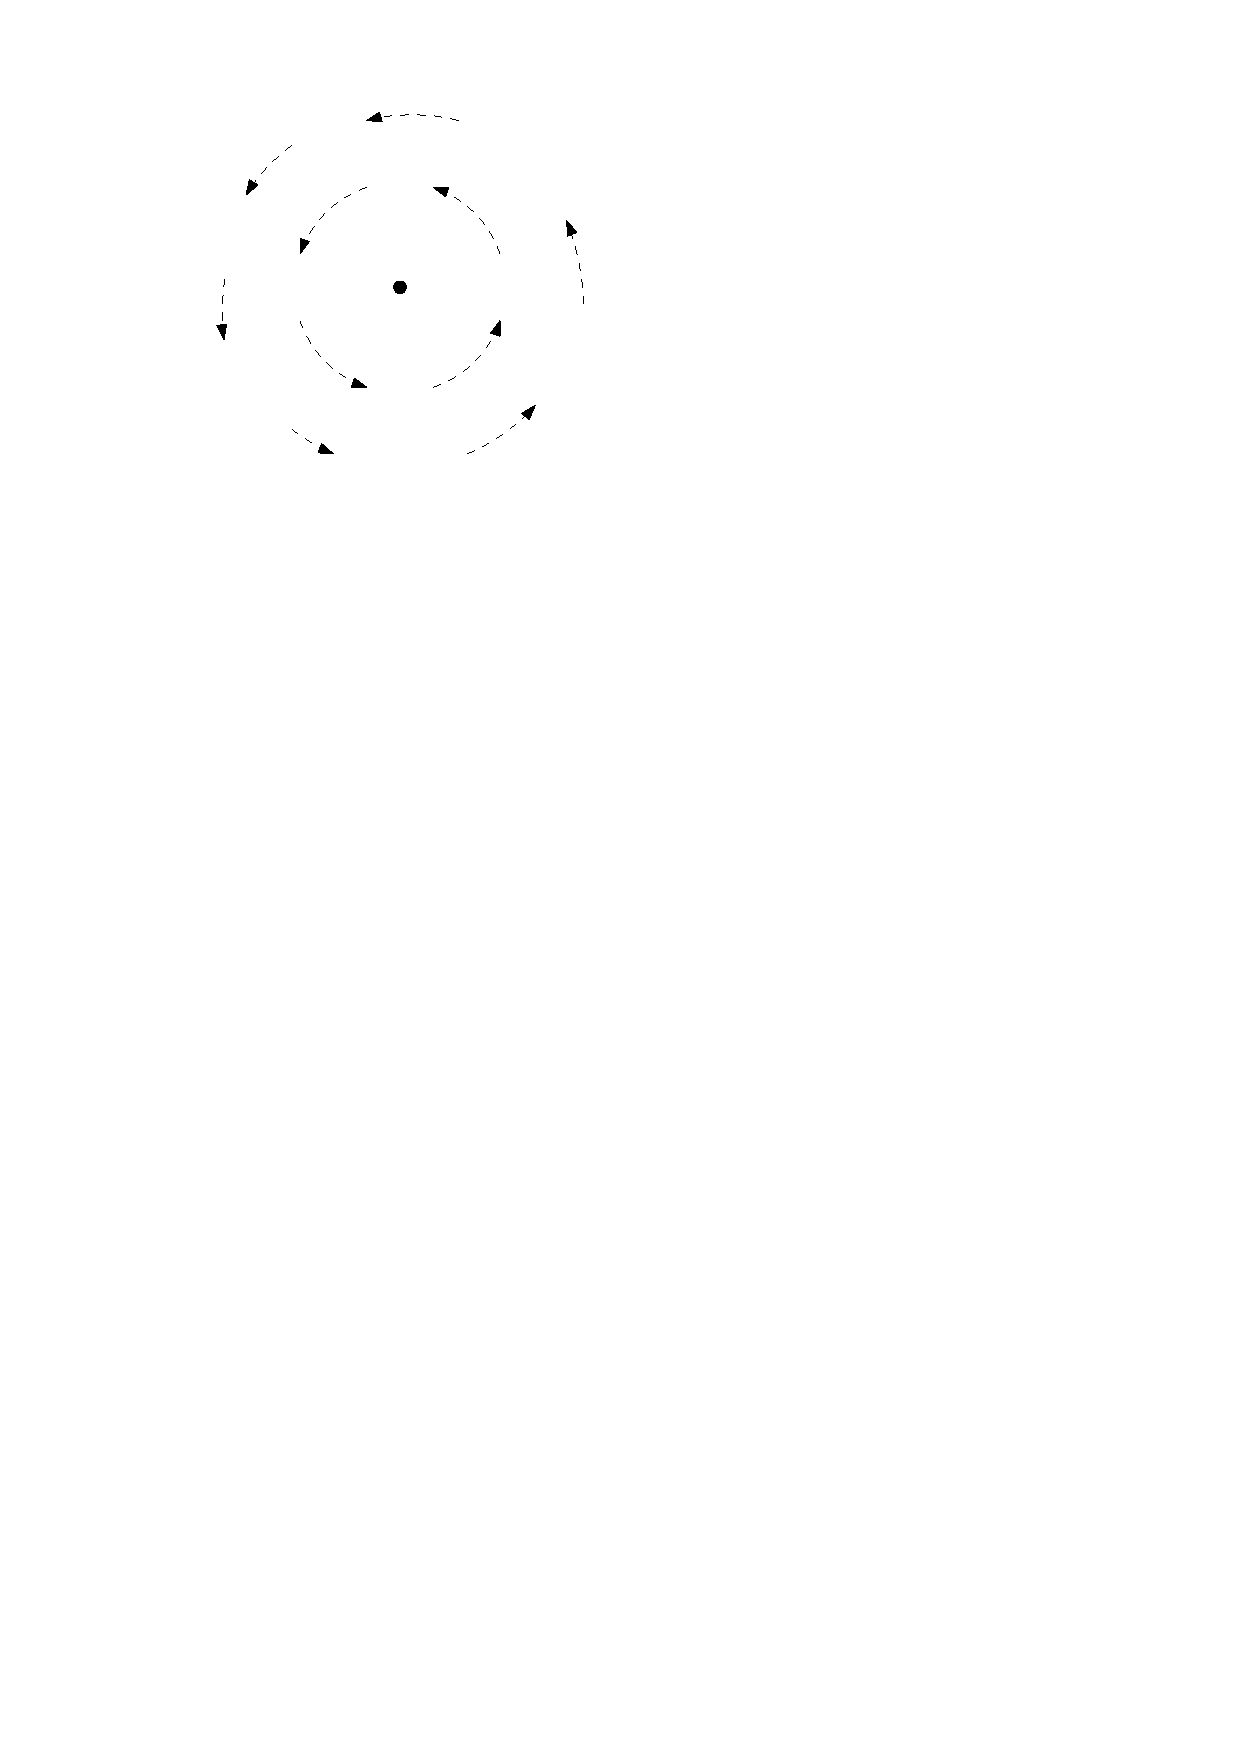
\includegraphics[scale=0.7]{./7.3 Flusso irrotazionale/7.3-4}
		\centering
		\caption{Vortice}
	\end{figure}
%

Si considera poi $n = 1$.

\subsubsection{Corrente parallela}
Questo risulta essere una velocità costante nella direzione $x$, volendo è possibile orientarne l'angolo:
%
	\begin{equation*}
		\phi = A r \cos{\theta} = x \rightarrow \grad{\phi} = A \hat{\imath}_x
	\end{equation*}
%
 %
	\begin{figure}[ht]
		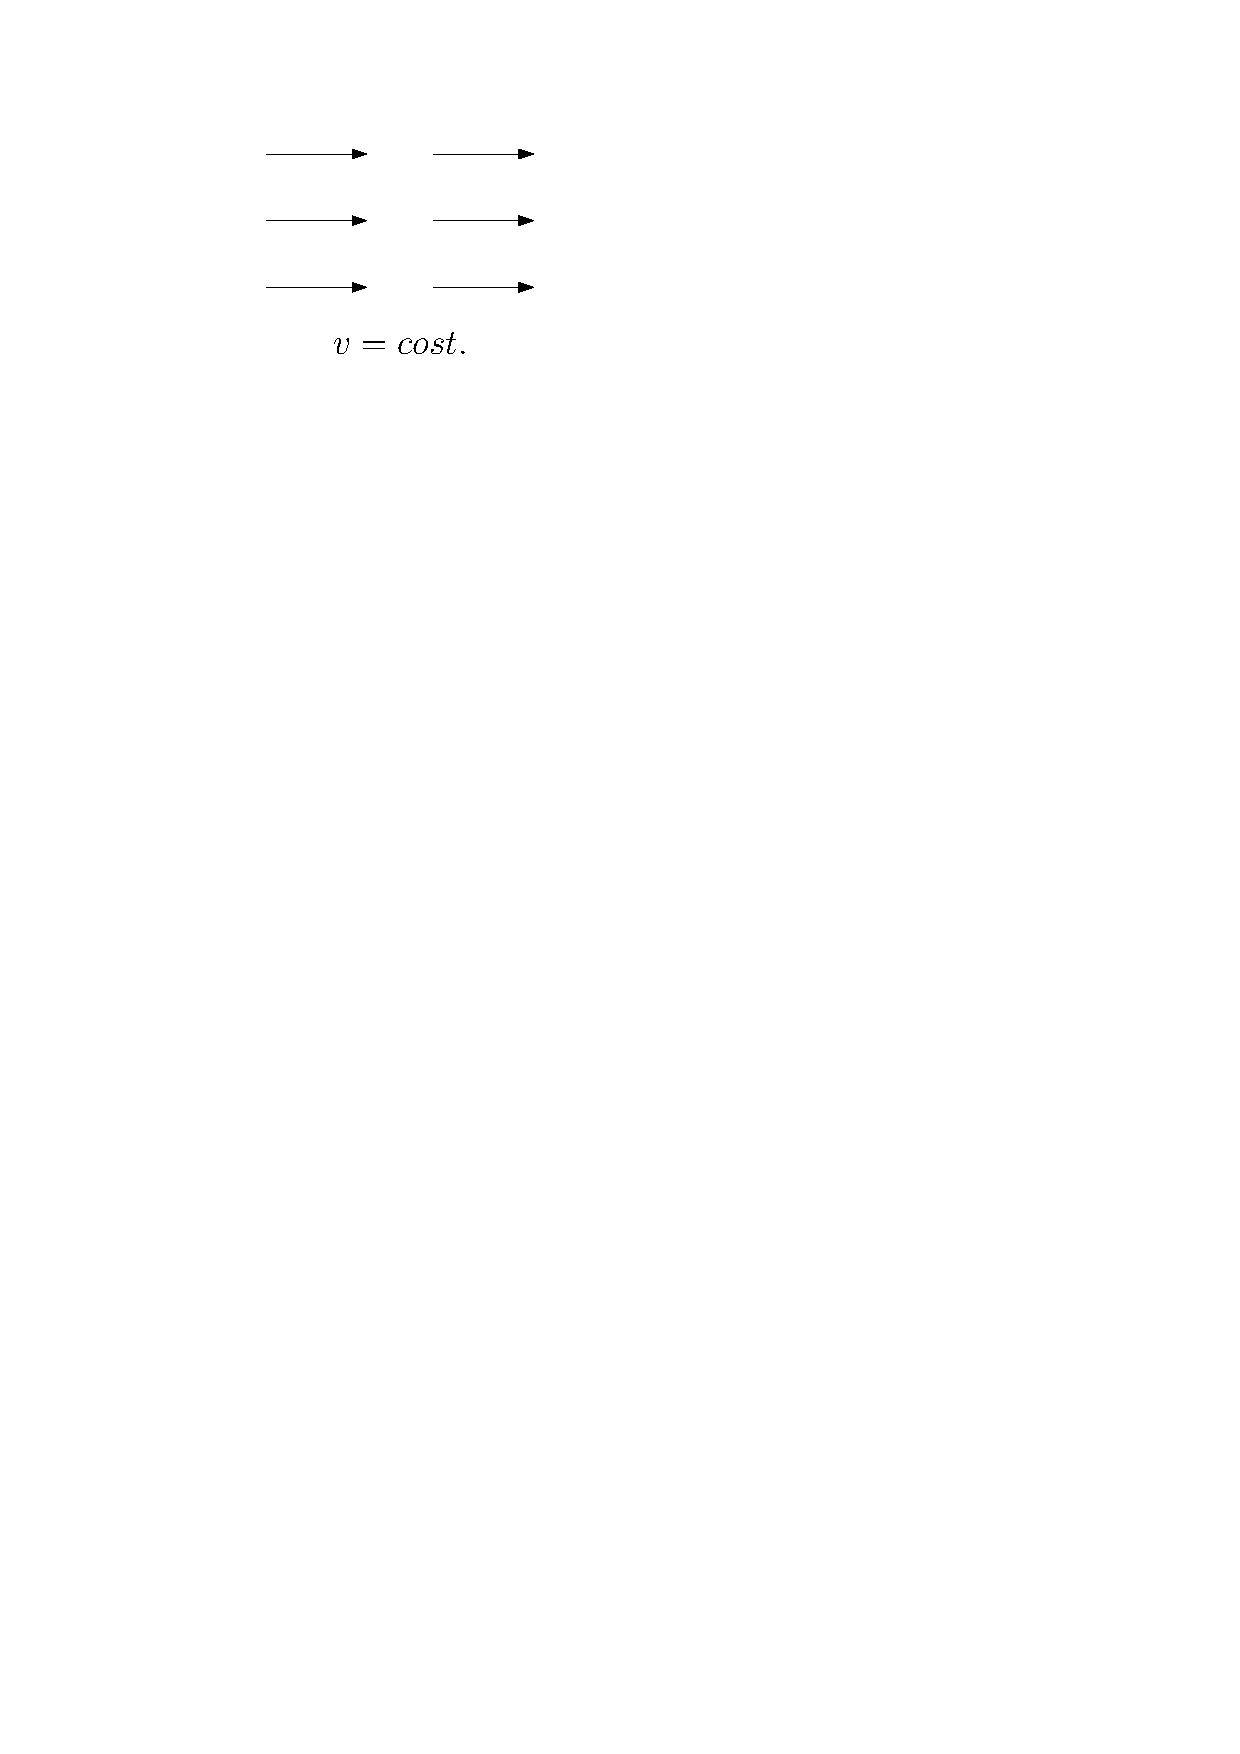
\includegraphics[scale=0.7]{./7.3 Flusso irrotazionale/7.3-4-2}
		\centering
		\caption{Velocità costante}
	\end{figure}
%

\subsubsection{Dipolo}
Si ottiene un dipolo, cioè le linee di corrente sono tutte delle circonferenze.
Accade praticamente solo in casi teorici, è interessante più che altro per combinarlo con altre soluzioni.
%
	\begin{equation*}
		\begin{gathered}
			\phi = A r^{- 1} \cos{\theta}\\
			 \grad{\phi} = - r^{- 2} \hat{\imath}_r \cos{\theta} - r^{- 2} \sin{\theta} \hat{\imath}_\theta
		\end{gathered}
	\end{equation*}
%
 %
	\begin{figure}[ht]
		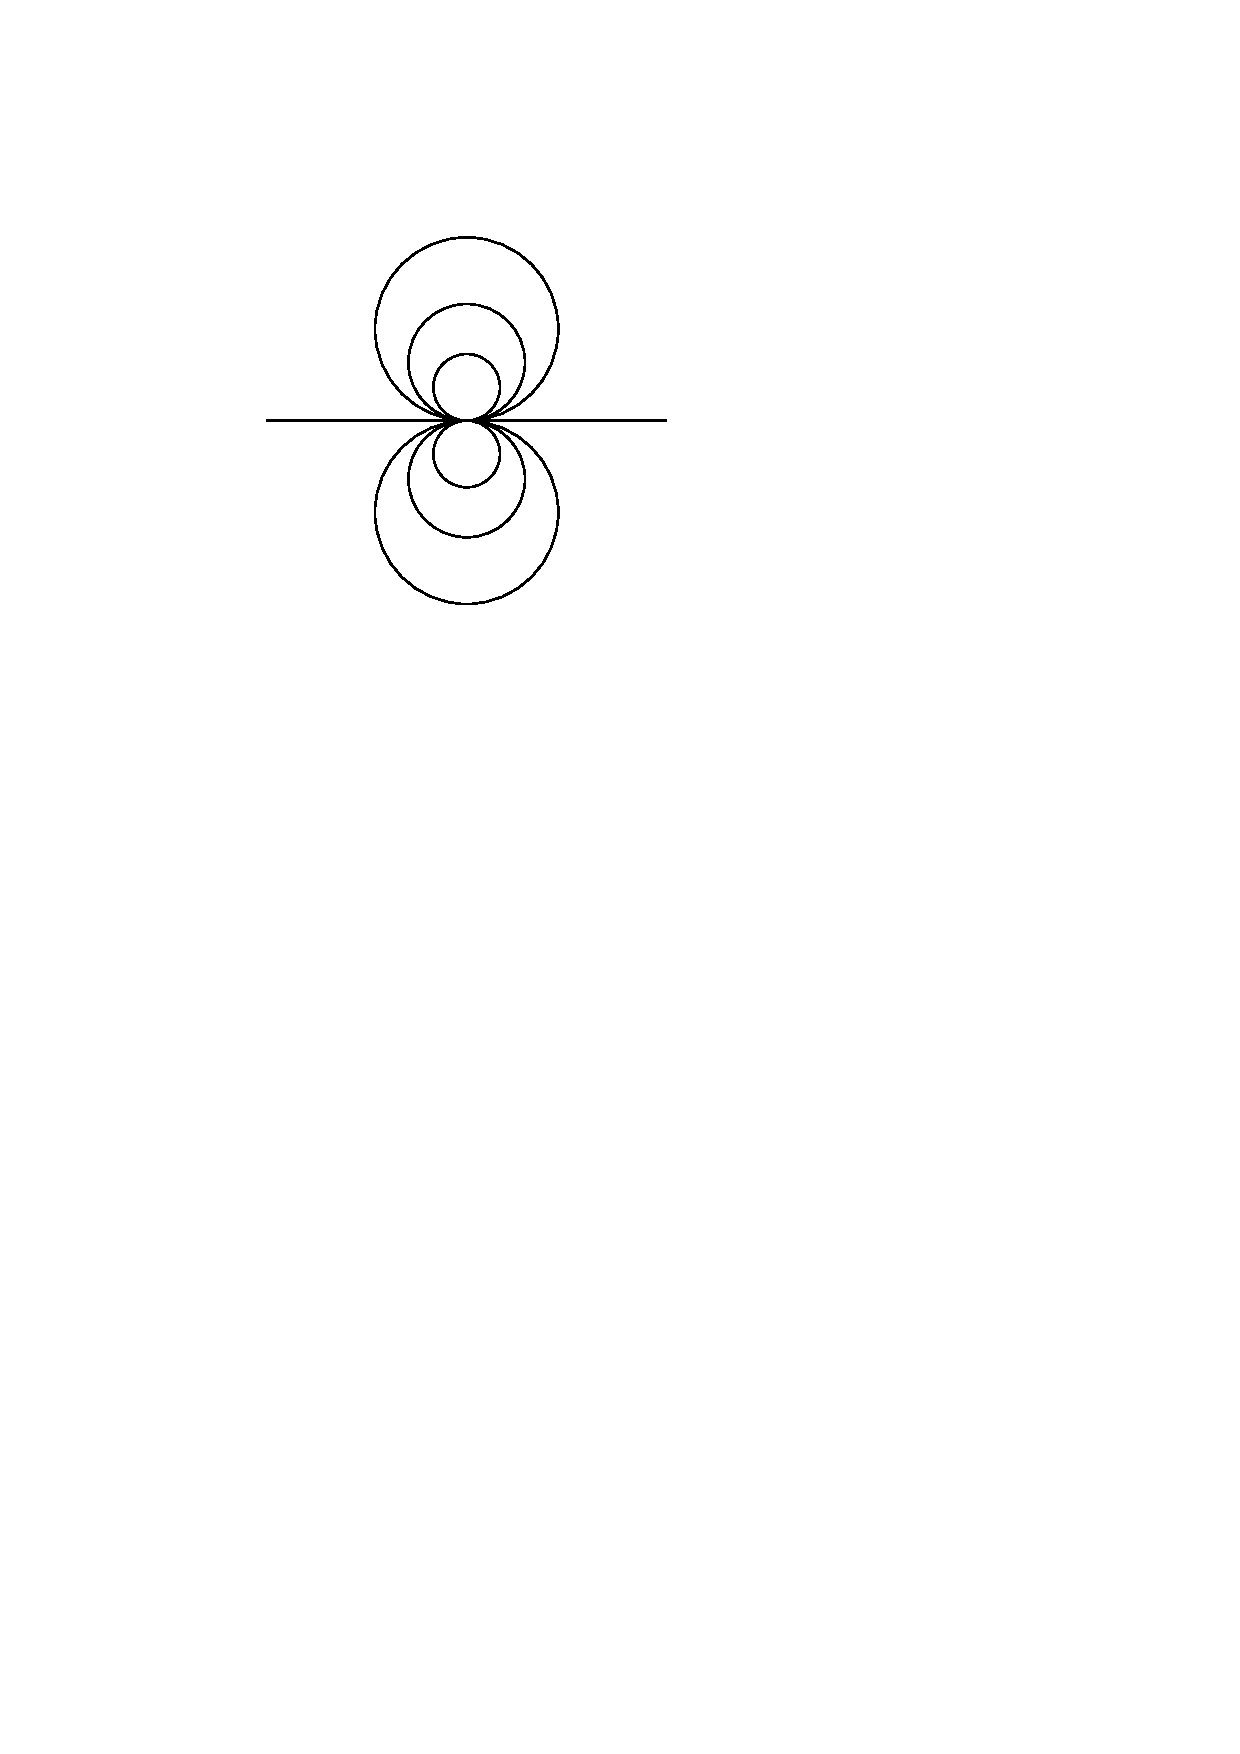
\includegraphics[scale=0.7]{./7.3 Flusso irrotazionale/7.3-5}
		\centering
		\caption{Dipolo}
	\end{figure}
%

\subsubsection{Corrente su un cilindro}
Le soluzioni di cui prima possono essere combinate, ad esempio si vede che combinando dipolo e velocità costante si ottiene il moto attorno ad un cilindro:
%
	\begin{equation*}
		\begin{gathered}
			\phi = A \left( r + \frac{1}{r} \right) \cos{\theta}\\
			\pdv{\phi}{r} = A \left( 1 - \frac{1}{r^r} \right) \cos{\theta}\\
			\frac{1}{r} \pdv{\phi}{\theta} = A \left( 1 + \frac{1}{r^r} \right) (-\sin{\theta})
			\pdv{\phi}{r} = 0
		\end{gathered}
	\end{equation*}
%
Notare che per $\pdv{\phi}{r} = 0$ sulla circonferenza la normale è nulla.
%
	\begin{figure}[ht]
		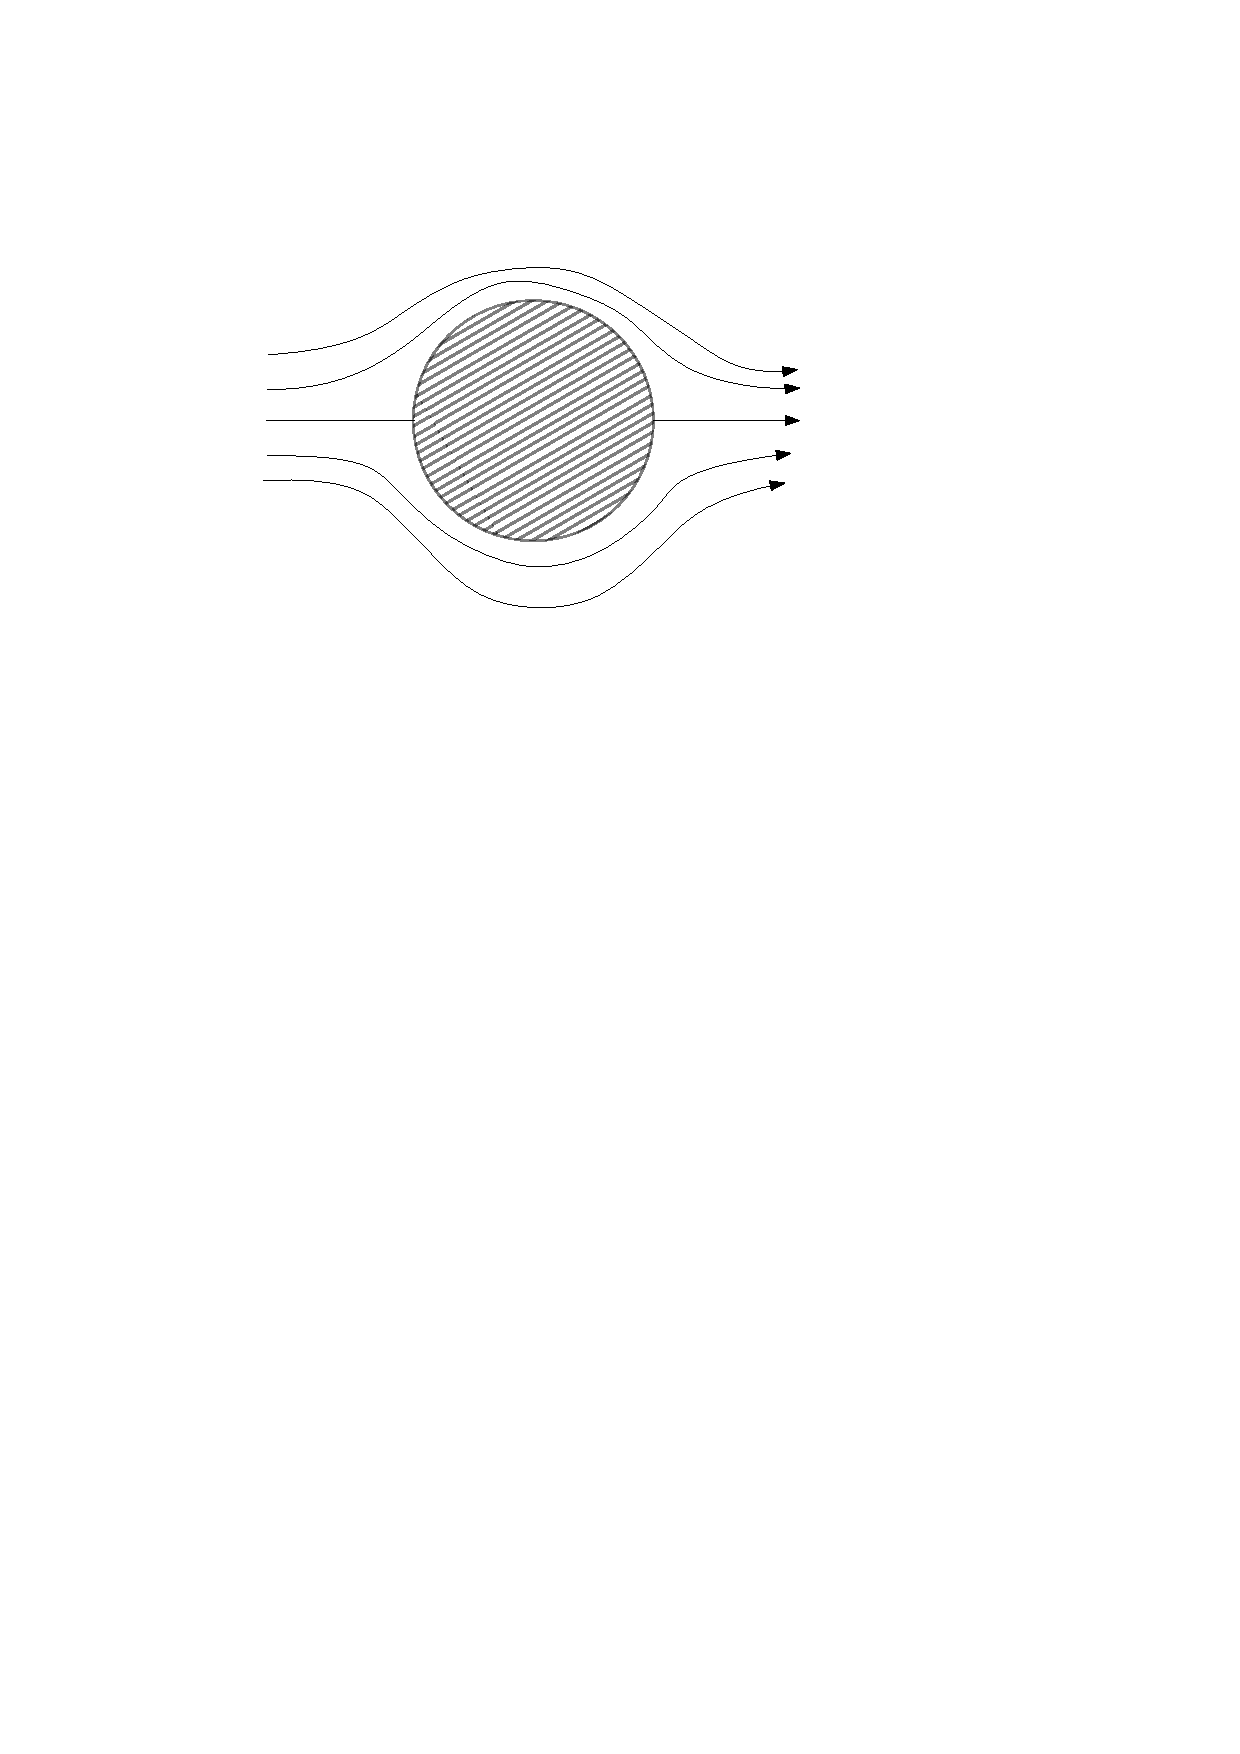
\includegraphics[scale=0.7]{./7.3 Flusso irrotazionale/7.3-6}
		\centering
		\caption{Flusso attorno ad un cilindro}
	\end{figure}
%
Si sarebbe potuto ottenere lo stesso risultato tramite la funzione di corrente.
Si inizia definendo un potenziale:
%
	\begin{equation*}
		\begin{gathered}
			\pdv{\phi}{x} = u\\
			\pdv{\phi}{y} = \theta
		\end{gathered}
	\end{equation*}
%
Si definisce poi la funzione di corrente:
%
	\begin{equation*}
		\begin{gathered}
			\pdv{\psi}{y} = u\\
			\pdv{\psi}{x} = v
		\end{gathered}
	\end{equation*}
%
Confrontando quindi il caso precedente e questo si ottiene che:
%
	\begin{equation*}
		\begin{gathered}
			u_x + v_y = 0 \rightarrow \laplacian{\phi} = 0\\
			u_y - v_x = 0 \rightarrow \laplacian{\psi} = 0
		\end{gathered}
	\end{equation*}
%
Risulta sempre l'equazione di Laplace, ma cambia la relazione che esprime.
Per simmetria in questo caso sulla circonferenza non agiscono forze.

\subsubsection{Paradosso di D'Alambert}
Come appena visto quindi sulla circonferenza non dovrebbero esserci forze, eppure effettuando esperimenti si vede che le forze risultanti non sono nulle.
È il cosiddetto paradosso di D'Alambert, che si spiega con il fatto che in realtà il moto non è del tutto irrotazionale ma c'è una scia, oltre che con le considerazioni di seguito.
%
	\begin{figure}[ht]
		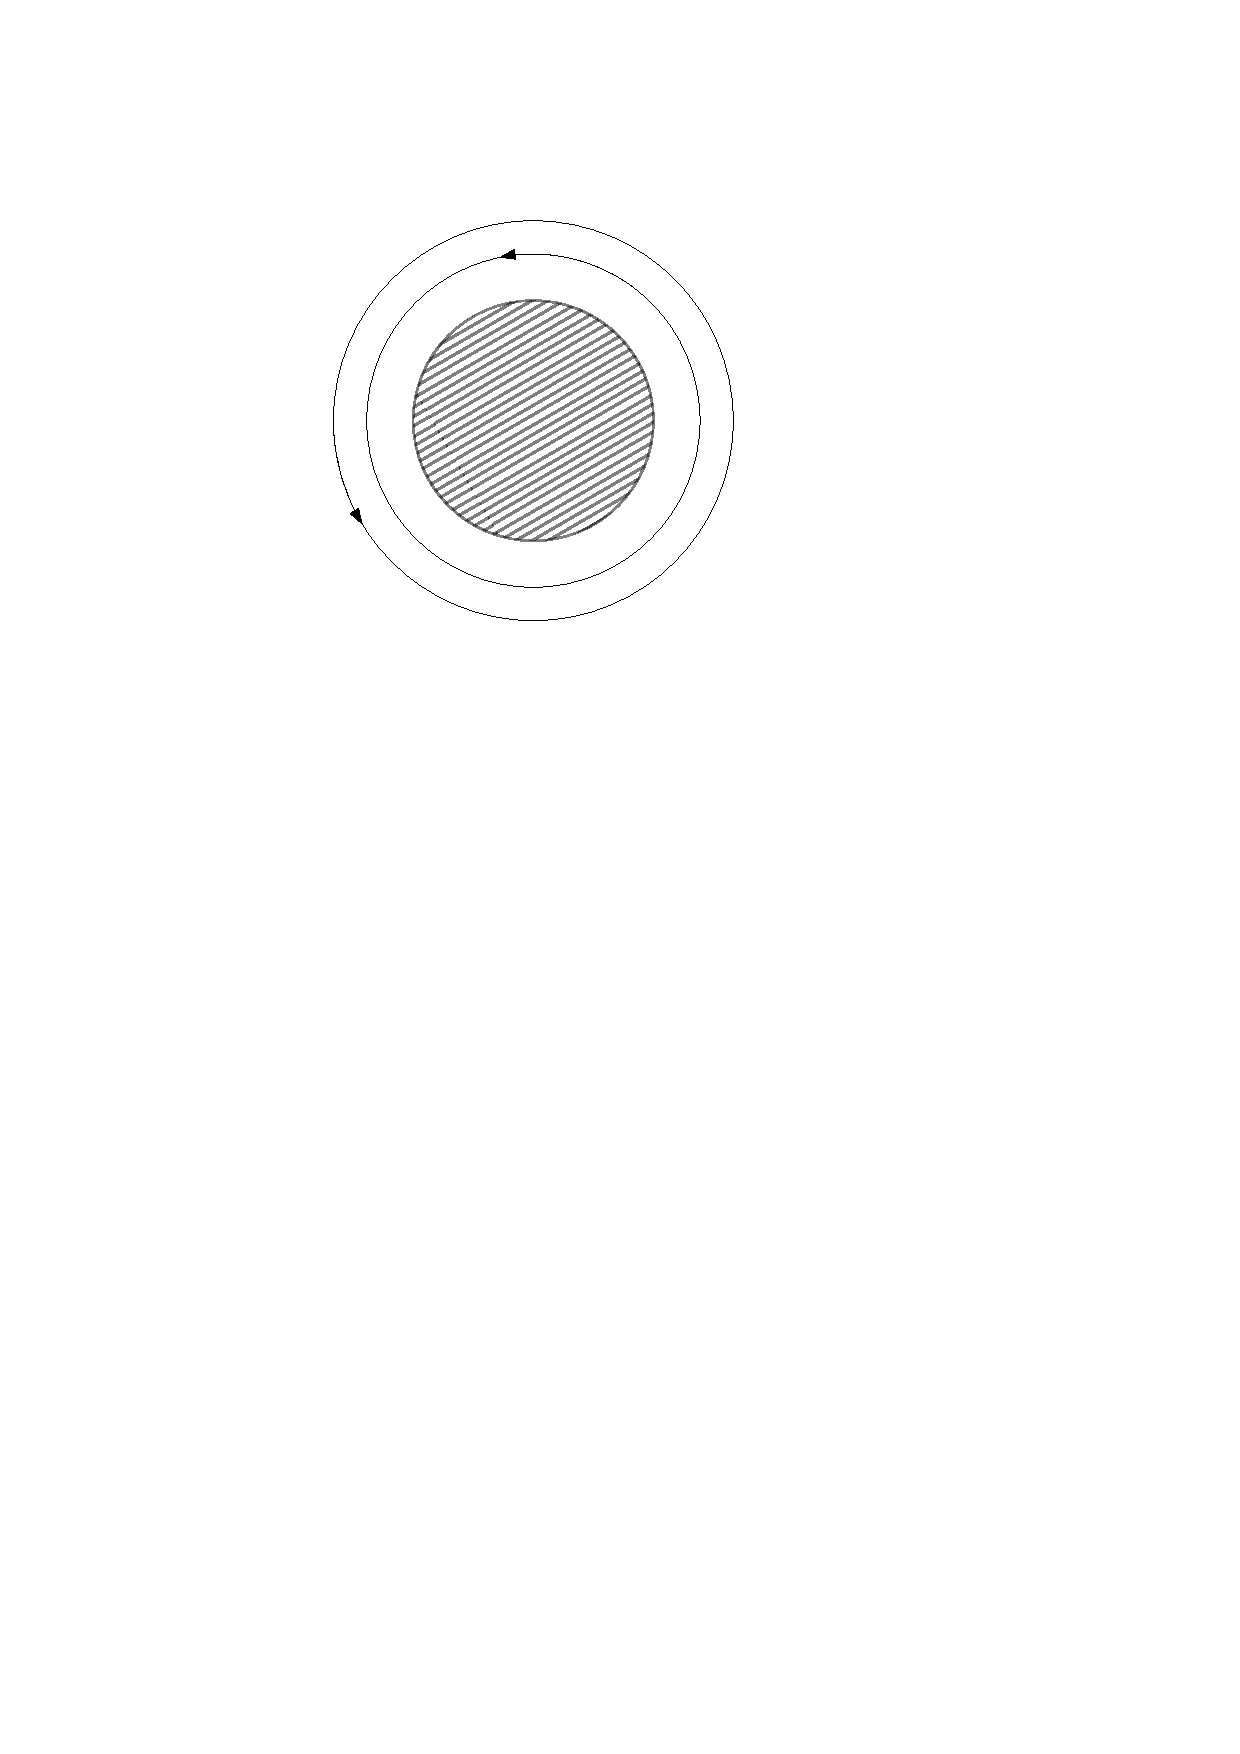
\includegraphics[scale=0.7]{./7.3 Flusso irrotazionale/7.3-7}
		\centering
		\caption{Moto irrotazionale attorno ad un cerchio}
	\end{figure}
%
Si parte considerando che un vortice è una soluzione valida per un moto irrotazionale attorno ad un cerchio:
%
	\begin{equation*}
		\phi = B \theta
	\end{equation*}
%
E in generale è possibile fare una combinazione del tipo:
%
	\begin{equation*}
		\psi = A \left( r + \frac{1}{r} \right) \cos{\theta} + B \theta
	\end{equation*}
%
L'applicazione delle condizioni al contorno permette di determinare solamente un coefficiente:
%
	\begin{equation*}
		v_\infty = A \vec{i}_x \quad B ?
	\end{equation*}
%
Quindi la soluzione per un moto irrotazionale attorno ad un cerchio non è unica.
È indeterminata a meno di un vortice, aggiungendo questo alla soluzione vista prima si ha che le linee di corrente cambiano.
 %
	\begin{figure}[ht]
		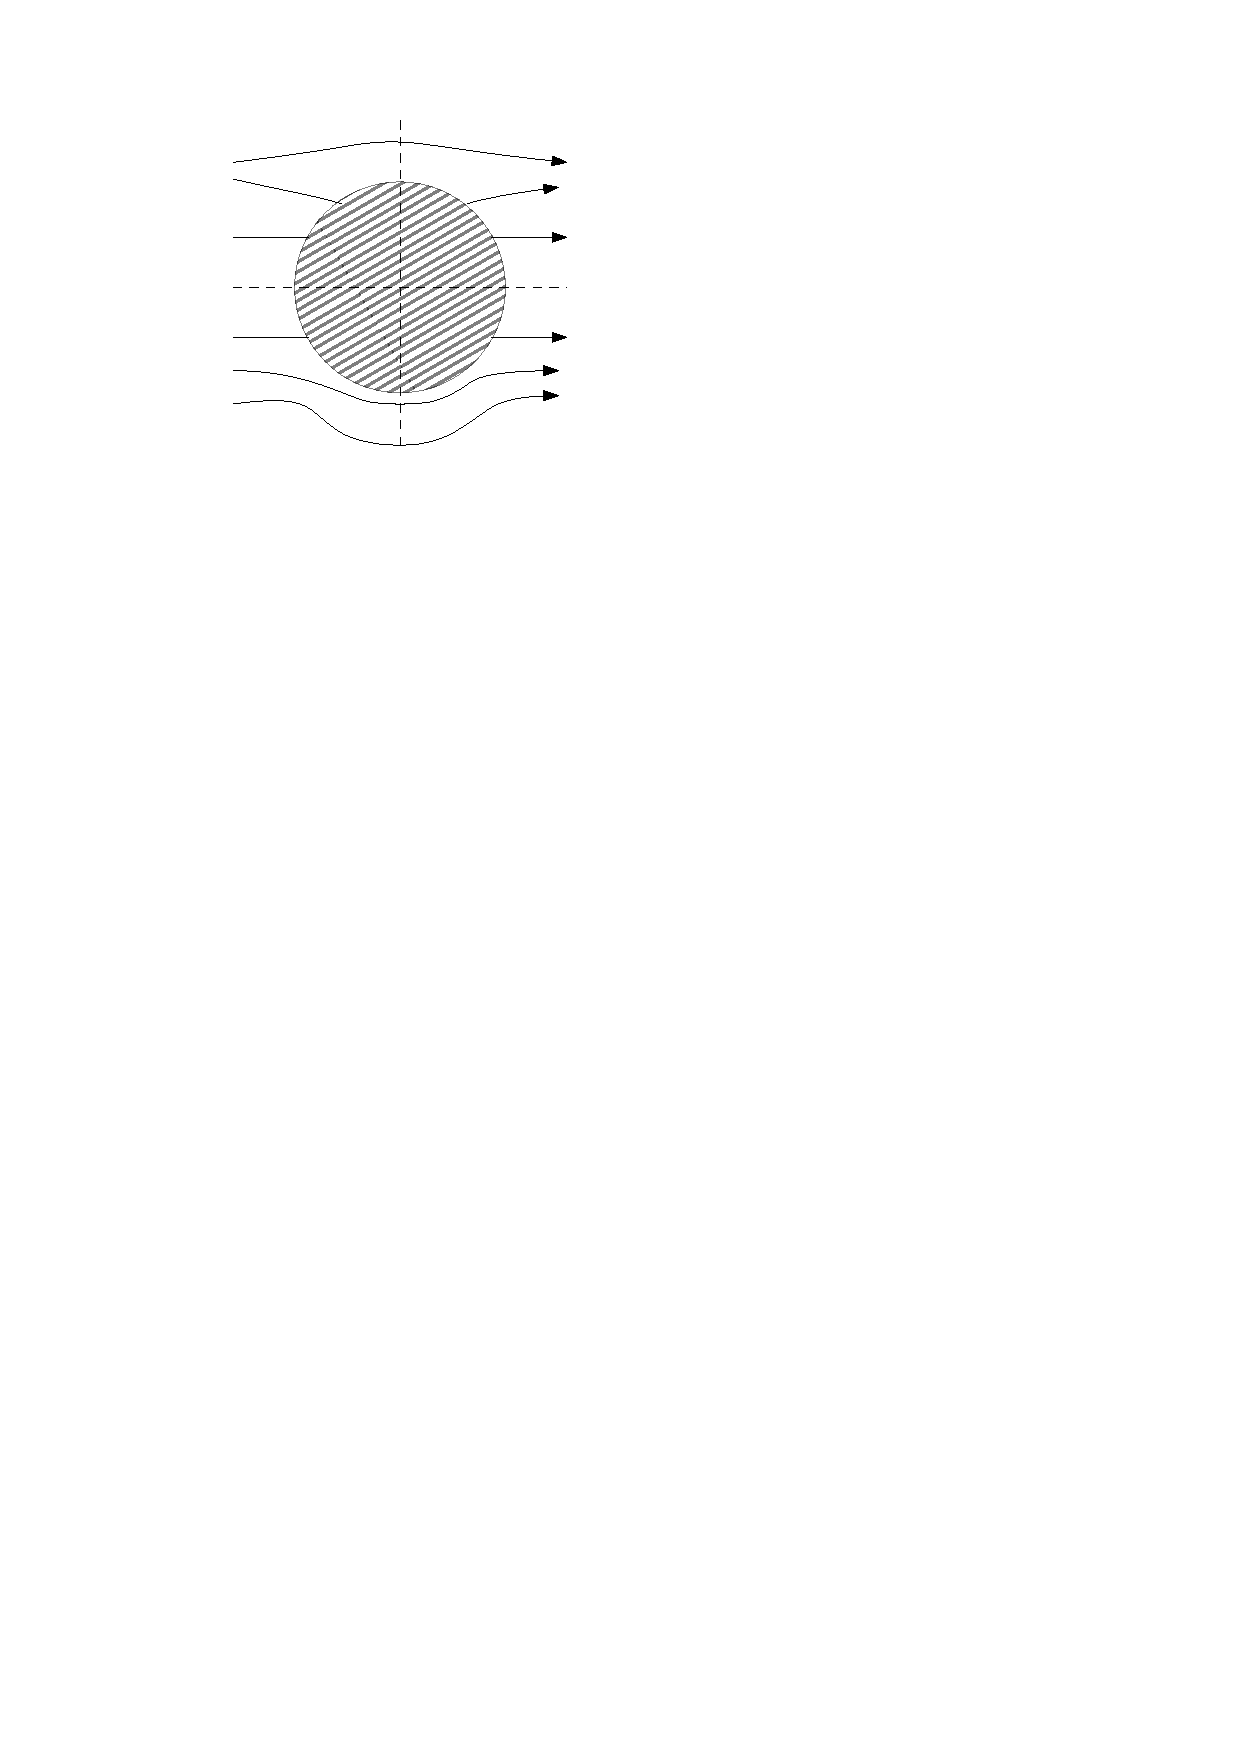
\includegraphics[scale=0.8]{./7.3 Flusso irrotazionale/7.3-8}
		\centering
		\caption{Linee di corrente attorno ad un cerchio}
	\end{figure}
%
Visto che le linee di corrente non sono più simmetriche, questo permette che ci sia una forza per via della differenza di pressione.


Detta portanza la componente $F_y$ ortogonale a $\uline{v}_\infty$, si può dimostrare che è legata $B$ del vortice, o meglio alla circolazione:
%
	\begin{equation*}
		F_y = \rho \Gamma \uline{v}_\infty
	\end{equation*}
%
Vi è anche una $F_x$, componente parallela a $\uline{v}_\infty$, detta resistenza.
Quest'ultima è importante dato che il lavoro è dato da $\uline{F} \vdot \uline{v}_\infty$.
In applicazioni come aerei etc. si vuole indurre una circolazione per massimizzare la portanza ed evitare separazione e scia che invece aumentano la resistenza.

\subsection*{Bibliografia 7.3}
\cite[Cap.\ 10.4]{CengelCimbala}\\
\cite[Cap.\ 10.2, 10.3]{PnueliGutfinger}